\documentclass[10pt]{article}
\usepackage[utf8]{inputenc}
\usepackage[T1]{fontenc}
\usepackage[english]{babel}
\usepackage{amsfonts}
\usepackage{amsmath}
\usepackage[pdftex]{color,graphicx}
\usepackage{fancyhdr}
\usepackage{textcomp}
\usepackage{lmodern}
\usepackage{xcolor}
\usepackage{multicol}
\usepackage{soul}
\usepackage{algorithmic}
\usepackage{wrapfig}
\usepackage{float}
\usepackage{mdwlist}
\usepackage{pgfgantt}
%\usepackage{hyperref}
\pagestyle{fancy}
\newcommand{\HRule}{\rule{\linewidth}{0.5mm}}

%If in need of a header for the document, uncomment this and add desired text!
%\fancyhead[LO,LE]{}
%\fancyhead[RO,RE]{}
%%%%%%%%%%%% END OF PREAMBLE %%%%%%%%%%%%%%%%%%%%%%%%%%%%%%%%%%%%
\begin{document}
\begin{titlepage}

\begin{center}

\textsc{\LARGE DATANET}\\[1.5cm]

%\textsc{\Large Datanet}\\[0.5cm]

\HRule \\[0.4cm]

{ \bfseries Weekly assignment 2}\\[1cm]
%\includegraphics[width=0.8\textwidth]{carrie}\\[0.1cm]

\HRule \\ [7.5cm]

% Author and supervisor
\begin{minipage}{0.5\textwidth}
\begin{flushleft} \large
Martin Jørgensen (tzk173)\\
\textit{martinnjorgensen@gmail.com}\\
\end{flushleft}
\end{minipage}
\begin{minipage}{0.4\textwidth}
\begin{flushright} \large
\textbf{\today} \\
\end{flushright}
\end{minipage}

\vfill

% Bottom of the page front page


\end{center}

\end{titlepage}
\clearpage

\section{Theoretical part}
\subsection{Domain Name System}
\subsubsection{DNS provisions}
\begin{enumerate*}
  \item \textbf{Fault tolerance:} There are 13 root DNS server, which gives
        great redundancy, futhermore the TLD servers whose addresses are stored
        on the root servers are usually cached on local computers.
  \item \textbf{Scalability:} Since everyone can basically add a DNS server to
        the system, simple by adding them in the TLD servers, it is very
        scalable.
  \item \textbf{Efficiency:} The \texttt{RR}'s can be cached for a period of
        time, meaning a user don't need to do the DNS lookup everytime they need
        to resolve a hostname.
\end{enumerate*}

\subsubsection{DNS lookup and format}
\begin{enumerate}
  \item \textbf{Part 1:} The \texttt{CNAME} record can be used for loadbalancing
        simply by adding several canonical names for the same address. The DNS
        server will then rotate the list of addresses each time the canonical
        name is looked up.
  \item \textbf{Part 2:} \textit{Iterative} DNS lookups is when the DNS server
        answers the client that it does not ahve the answer, but that the client
        should send a request to another, specified nameserver.
        \textit{Recursive} DNS lookup is when the DNS server performs the next
        lookup for the client and then returns the answer.
  \item \textbf{Part 3:}
        The first thing that will happen is that the students machine will query
        the local DNS about \texttt{grooveshark.com}.
\begin{verbatim*}
; <<>> DiG 9.9.2-P2 <<>> grooveshark.com +recurse +trace +answer +nodnssec
;; global options: +cmd
.			15954	IN	NS	g.root-servers.net.
.			15954	IN	NS	b.root-servers.net.
.			15954	IN	NS	e.root-servers.net.
.			15954	IN	NS	h.root-servers.net.
.			15954	IN	NS	d.root-servers.net.
.			15954	IN	NS	a.root-servers.net.
.			15954	IN	NS	j.root-servers.net.
.			15954	IN	NS	f.root-servers.net.
.			15954	IN	NS	k.root-servers.net.
.			15954	IN	NS	c.root-servers.net.
.			15954	IN	NS	i.root-servers.net.
.			15954	IN	NS	m.root-servers.net.
.			15954	IN	NS	l.root-servers.net.
;; Received 239 bytes from 8.8.8.8#53(8.8.8.8) in 332 ms
\end{verbatim*}
      The root servers will then, using their own records of the GTLD servers,
      go on to ask the \texttt{com} GTLD server for \textit{grooveshark.com}.
\begin{verbatim*}
com.			172800	IN	NS	l.gtld-servers.net.
com.			172800	IN	NS	g.gtld-servers.net.
com.			172800	IN	NS	m.gtld-servers.net.
com.			172800	IN	NS	i.gtld-servers.net.
com.			172800	IN	NS	e.gtld-servers.net.
com.			172800	IN	NS	j.gtld-servers.net.
com.			172800	IN	NS	d.gtld-servers.net.
com.			172800	IN	NS	k.gtld-servers.net.
com.			172800	IN	NS	h.gtld-servers.net.
com.			172800	IN	NS	f.gtld-servers.net.
com.			172800	IN	NS	b.gtld-servers.net.
com.			172800	IN	NS	a.gtld-servers.net.
com.			172800	IN	NS	c.gtld-servers.net.
;; Received 532 bytes from 202.12.27.33#53(202.12.27.33) in 650 ms
\end{verbatim*}
      The GTLD server will then using their own records query the nameservers
      that are listed in \textit{grooveshark.com}'s NS records, query them for
      groovesharks address.
\begin{verbatim*}
grooveshark.com.	172800	IN	NS	ns1.grooveshark.com.
grooveshark.com.	172800	IN	NS	ns2.grooveshark.com.
grooveshark.com.	172800	IN	NS	ns3.grooveshark.com.
;; Received 146 bytes from 192.43.172.30#53(192.43.172.30) in 87 ms
\end{verbatim*}
      Finally the \textit{grooveshark.com} nameservers will then reply with the
      \texttt{A} record for \textit{grooveshark.com}.
\begin{verbatim*}
grooveshark.com.	60	IN	A	8.20.213.76
grooveshark.com.	86400	IN	NS	ns3.grooveshark.com.
grooveshark.com.	86400	IN	NS	ns1.grooveshark.com.
grooveshark.com.	86400	IN	NS	ns2.grooveshark.com.
;; Received 162 bytes from 8.20.213.44#53(8.20.213.44) in 260 ms
\end{verbatim*}
      The grooveshark nameserver will send that address to the GTLD nameserver,
      who will pass the answer on to the root server, who will pass it on to
      the local nameserver (in our case, google's) who in turn will pass it to
      the client, who now have the IP for grooveshark.com

      \noindent The above data was generated using the following command on a
      Linux system on eduroam:
      \texttt{dig grooveshark.com +recurse +trace +answer +nodnssec}
      the last switch, \texttt{+nodnssec} is just to clean up the output, since
      some of the servers responds with \texttt{RRSIG} keys for DNSSEC lookup.
\end{enumerate}


\subsection{Transport Protocols}

\subsubsection{TCP reliability and utilization}
\begin{enumerate}
  \item \textbf{Part 1:} The \texttt{ACK} packet in the last part of the
        hadnshake is not strictly needed since both ends of the connection
        have already acknowledged that they want to create the connection by
        sending the \texttt{SYN}, \texttt{SYNACK} packets. The \texttt{ACK}
        packet does also serve a practical purpose, it allows the attachment of
        a TCP payload, so for instance with HTTP, once the server have
        acknowledged the client, the client can send the request immediately.
  \item \textbf{Part 2:} TCP provides full duplex by providing a send- and a
        recieve buffer, data put in the writebuffer will then be send over the
        IP link layer at some point. There is no given interval where TCP must
        transmit these buffers, so there is not security for when this will
        happen. This read/write buffer system means that TCP users will percieve
        TCP as sending/recieving at the same time.
\end{enumerate}

\subsubsection{Reliability vs overhead}
\begin{enumerate}
  \item \textbf{Part 1:} The first overhead created by TCP is the
        \textit{3-way handshake},  since UDP does not do this handshake, it can
        can be considered overhead. Additional overhead is incured as a certain
        amount of data is stored and used when sending TCP traffic in order to
        manage framenumbers, sequencing and prevent dataloss and duplicates.
        Furthermore the 20byte TCP segment header is considerably larger than
        8byte UDP segment header, meaning each segment increases the total time
        spent by TCP over UDP.
  \item \textbf{Part 2:} Packets are always delivered in order, so if a packet
        does not arrive, the reciever will request that it be sent again,
        delaying the transfer of the following packets, but ensuring that all
        packets arrive, and that they arrive in the correct order.
\end{enumerate}

\subsubsection{Use of transport protocols}
\begin{enumerate}
  \item \textbf{DNS Part 1:} Both TCP and UDP can be used for DNS request, both
        will happen on port 53. The convention is to use UDP for normal DNS
        requests, but TCP can be used as well, but it does have worse
        performance. Zone transfers should always be done in TCP since the loss
        of records qould be quite fatal.
  \item \textbf{DNS Part 2:} TCP could help prevent cachepoisoning since the TCP
        segment header contains a framenumber, that is generated on both
        endpoints of the connection, this helps prevent man in the middle
        attacks since he will have to know framenumbers for both participants.
        If an ISP DNS server is succesfully poisoned, it will mean that ALL the
        customers of that ISP who do not have the affected domain cached will be
        poisoned. Amongst ISP customers are other potential nameservers, meaning
        that the poisoned cache entry will spread to other nameservers over
        time.
  \item \textbf{Simple HTTP requests and responses}
        \begin{enumerate*}
          \item There will be used 8 packets for the entire exchange.The
            following transaction will happen:
            \begin{itemize*}
              \item Client sends \texttt{SYN} packet
              \item Server responds \texttt{SYN-ACK} packet
              \item Client responds \texttt{ACK} packet with TCP payload
                    containing the request.
              \item The server responds with the 304 HTTP response.
              \item Client sends \texttt{FIN} packet
              \item Server sends \texttt{ACK} packet
              \item Server sends \texttt{FIN} packet
              \item Client sends \texttt{ACK} packet
            \end{itemize*}
            After the final \texttt{ACK} packet, both close the connection.

          \item Technically there is only 2 packets containing data, the request
                and the response. The 6 other packets are only there to
                facilitate handshake and close the connection.
                To justify the use of TCP is the fact if the response or request
                gets lost, the entire transaction is ruined. The only way to
                judge that would be to implement a timeout, which could mean
                long loading times.

          \item UDP could be used as a transport protocol for HTTP, but using
                the argument from above, I would argue it is a bad idea.

        \end{enumerate*}
\end{enumerate}


\subsection{TCP: Principles and practice}
\subsubsection{TCP headers}
\begin{itemize}
  \item \textbf{Part 1.1:} The \texttt{RST} bit is the source telling the
        recipient to immidietley reset/close the connection. This might be send
        if the client tries to communicate on a closed port, then the host will,
        depending on configuration, send a \texttt{RST} packet back, or ignore
        the connection.
  \item \textbf{Part 1.2:} The sequence and ACK-numbers are used to synchronise
        the TCP stream for both host and client, to ensure that all packet
        arrive and that they arrive in the correct fassion.
  \item \textbf{Part 1.3:} The windows size is the amount of data the sender is
        currently willing to recieve. The unit used us usually byte but could be
        anything.
  \item \textbf{Part 1.4:} When the window size reaches zero the sender will no
        longer recieve segments. This means that the only segments that can get
        through is those with the \texttt{ACK}, \texttt{RST} or \texttt{URG}
        bits send. This is used for flow control since it allows for updates of
        the window size.
  \item \textbf{Part 2.1:} The server would need to send the synced sequence
        number and window size in the pack to tell the client how much data
        it's allowed to send.
  \item \textbf{Part 3.1:}\\
        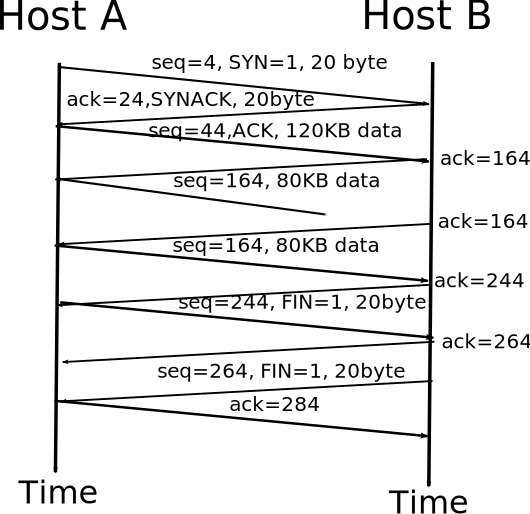
\includegraphics[width=\textwidth]{transmission.png}
\end{itemize}

\subsubsection{High performance TCP}
\begin{enumerate}
  \item The max number for window size is 65535bytes. This limit is imposed by
        the 16bit length if the window field, which means that each packet can
        only ever be \~65KB.
  \item Throughput as a function of recieve window size and RTT can be found by
        the following ineqation:
        \[
            \text{throughput} \leq \frac{\text{window}}{\text{RTT}}\\
            100.000.000B/s \leq \frac{2^{16}-1}{RTT}
        \]
        Solving for the $RTT$ wil then give us:
        \[
            RTT = 0,00065535s = 0,6ms
        \]
        Any roundttrip time above that will limit the throughput with the 16-bit
        window size on a 100Mb/s connection.
  \item Solving this ineqation will give the needed window size:
        \[
            100.000.000B/s \leq \frac{window}{0.072s}\\
            window = 72.000.000B
        \]
        The needed scale would then be around 1098.
        A header that can fully utilize the $100MB/s$ could look like this:\\
        \texttt{001000000010000000000001}
\end{enumerate}

\subsubsection{Flow and Congestion Control}
\begin{enumerate}
  \item \textbf{Part 1:} TCP employes 4 types of congestion control:
        \textit{Slow-start}, \textit{Congestion-avoidance},
        \textit{Fast-retransmit} and \textit{Fast-recovery}. Neither is network
        assisted since they're calculated exclusively by the sender (Slow-start
        \& congestion-avoidance) and the reciever (fast-retransmit \&
        fast-recovery)
  \item \textbf{Part 2:} By adjusting the amount of segments transmitted at a
        time, based on the segment size of the host and the congestion window
        variable.
  \item \textbf{Part 3:} The size is infered by the IW variable, which is
        calculated based on these conditions:
\begin{verbatim*}
If SMSS > 2190 bytes:
       IW = 2 * SMSS bytes and MUST NOT be more than 2 segments
If (SMSS > 1095 bytes) and (SMSS <= 2190 bytes):
       IW = 3 * SMSS bytes and MUST NOT be more than 3 segments
If SMSS <= 1095 bytes:
       IW = 4 * SMSS bytes and MUST NOT be more than 4 segments
\end{verbatim*}
        The text is copied directly from
        rfc5681\footnote{http://tools.ietf.org/html/rfc5681}. SMSS is the
        maximum segment size of the sender. IW is the initial  window size
        (the congestion windows initial size.)
  \item \textbf{Part 4:} \textbf{TODO!!} %TODO FIXME
\end{enumerate}



\section{Practical Section}

\subsection{Question 1}
Since all of the commands, will in all likelyhood (except perhaps
userlist for crowded servers) will fit within a single packet, and all
communication is done in clear text, the protocol becomes easily
readable for outsiders. The fact that the client and server
communicate in in human phrases like \texttt{HELLO}, \texttt{BYE} and
\texttt{LOOKUP} etc, means it's a bit like listening to an english
conversation. To my knowledge there is no easy way to avoid this,
except changing to an encoded or encryptet format, but this is not
socket based.

\subsection{Question 2}
No it is not fully robust. The fact that the server only uses one
thread is a limitation, since the thread have to alternate between
establishing new connections and communicating on existing ones, it is
``easy'' to clog up a socket, and it becomes easier as load increases.
Also, since the nameserver do not have a timeout limit for connection,
a crook can just connect a lot of new peers without keeping them
active and the information the server would have to save would keep
eating more and more resources. The damage done by ommiting the
message-end-marker is depending on how \texttt{select} determines of a
socket is ready to be read. If it waits for the marker before
returning the socket, then it would do no harm except fill up the
recieve buffer for that TCP connection. If \texttt{select} does not
wait for it but just sees that there is data in the buffer, it means
the server would hang, since \texttt{socket.recv} is a blocking call.

\subsection{Question 3}
The simplest way for the server to keep track of active peers it for
it to send a message to each peer once in a while (like the FTP
keep-alive message) and remove any peers that do not respond within a
given time. Alternatively one could make it the responsibility of the
peer to ``check in'' every once in a while to let the server know that
they are alive.

\subsection{Question 4}
A clear advantage of a centralised name server is control, both the
ability to shape trafiic, restrict peers from viewing each other, but
also to take statistics of usage.

A disadvantage is that if the name server gets attacked or taken down,
peers will only be able to talk to peers they already know, assuming
that a nick's IP gets saved at the peer end once the first message is
sent/the name is looked up.

To prevent such a thing, the name server should only be responsible
for authenticating nicknames, the IP/nickname table should be split up
and sent to the peers for safekeeping. This could be done by using
distributed hashtables. If a peer do not posses the address of the
nick they wish to speak to, they can ask all the peers in their own
table, and they can do the same, resulting in a ``recursive-dns'' like
lookup.


\end{document}